\chapter{Methods}
The model fitting process was validated by developing a simulation from which parameters of theta, migration rate and niches could be retrieved. A specifically designed laboratory experiment was commenced in January 2020 to test the model's theories in relation to microbial community dynamics. Due to the COV-19 pandemic the laboratory experiment was ended in March 2020. An alternative approach was devised, in which the model was fit to microbial species-area datasets compiled from the literature.

\section{Laboratory Experiment}

\subsection{Study area and sample collection}
\noindent

Soil was collected on site at Silwood Park, Berkshire, UK. Silwood Park comprises a variety of habitats including woodland, wetlands, heathland and formerly arable land \cite{CrawleyMichaelJ2005TfoB}. Soil types across the site consist of sandy or silty loam, with pH ranging from 4 to 6 \cite{LuckettKathryn2015Tbfr}. For this experiment soil was collected from a fallow field of acidic, sandy soil \cite{CrawleyMichaelJ2005TfoB}. Samples were acquired and sterilised during the first week of February. A total of 100 litres of soil was collected.

\subsection{Preparation of soil and mesocosms}
\noindent
The soil was homogenised by sieving and sterilising three times using an autoclave to destroy any present bacteria or fungi. We used five sizes of container: 0.2ml (PCR tube), 1.5ml (Eppendorf), 50ml (Fallon), 500ml and 5000ml. For each size of container 1, 2, 3, 4, 5 and maximum number of holes were made using a heated needle. Three replicates were made for each size of container and number of holes. The containers were then sterilised using the autoclave. The containers were filled with sterilised soil and sealed with an opaque lid. The containers were then buried on site, with sealed lids exposed and left to incubate for one month. 1.	If we use transparent covers for the tops of the tubes/containers this may create a gradient of light energy and moisture? Provide niches for heterotrophic and phototrophic microbes? Niche-based processes have been shown to be predominant in structuring observed aridity-related community patterns \cite{HuangMuke2019Iaas}. Abundance of predatory myxobacterial communities has also been correlated with temperature \cite{ZhouXiu‐Wen2014Mcia}.

\subsection{Soil properties measurements and climate data collection}
\noindent What is the pH of the soil where the samples were collected? pH of the soil where the samples were buried? pH has been show to affect microbial diversity \cite{GriffithsRobertI.2011Tbbo}.

\subsection{DNA extraction and sequence analysis}
\noindent After one month the containers were retrieved and DNA sampling was carried out the ZR Fungal/Bacterial DNA MiniPrep™ Isolation kit. Estimation of relative abundances of bacterial taxonomic groups was carried out using a previously defined PCR-based method \cite{FiererNoah2005Aosm}. Real-time PCR, or qPCR, allows for rapid quantitative assessment of soil microbial communities. I used 388 forward primer and 518 reverse primer as suggested for targeting all bacterial groups \cite{FiererNoah2005Aosm}. DNA samples from all 90 mesocosms were prepared for Illumina MiSeq 16S sequencing.

\section{Simulation}

\subsubsection{Overview}
This simulation is designed to mimic the process of island colonisation from a metacommunity. The colonisation process is constrained by migration rate and each island is characterised by number of niches and the size of each niche. The output of the simulation is the final community in each niche of each island, as well as a timeseries of species richness. 

\subsubsection{Metacommunity}
A metacommunity is generated at the beginning of the simulation using \textit{coalescence\_test} function, partially modified from a script provided by Dr James Rosindell. The function takes the input parameters: metacommunity size(\textit{J\_meta} = 50 000) and speciation rate (\textit{nu} = 0.001). Each run of the function produces 20 niche communities, each of size \textit{J\_meta}/20.  \bigskip

\noindent The function initialises a vector (\textit{lineages}) of length = \textit{J\_meta}/20 = \textit{niche\_size} with 1 as every value. An empty vector (\textit{abundances}) is initialised. The value of \textit{niche\_size} is given to \textit{N}. \textit{Theta} is calculated as \textit{nu*(niche\_size-1)/(1-nu)}. Then, while \textit{N $>$ 1}, a vector (\textit{linvect}) is created with values 1:length(\textit{niche\_size}). A random sample of \textit{linvect} is made (\textit{j}). A random decimal number is selected between 0 and 1 (\textit{randnum}). If \textit{rannum} is less than \textit{theta/(theta+N-1)}, then the value at \textit{lineages[j]} is appended to \textit{abundances}. Else, another random number (\textit{i}) is sampled from \textit{linvect}, excluding the last number selected. The values at \textit{lineages[i]} and \textit{lineages[j]} are summed and take the position of \textit{lineages[i]}. \textit{lineages[j]} is then removed from \textit{lineages}, so the vector is one value shorter. The value of \textit{N} is also decreased by 1. This repeats until \textit{N} = 1. The remaining value in the \textit{lineages} vector is added to \textit{abundances} and the function outputs a vector of simulated species abundances.\bigskip

\noindent At the end of the \textit{coalescence\_test} function, each of the 20 niches is assigned a letter type from A to T. A list of niche communities in the metacommunity is returned. It was chosen to generate no more than 20 niches within the metacommunity, because the simulation would not go beyond modelling 20 niches on an island. Any additional niches generated for the metacommunity would go unused. \bigskip

\noindent The \textit{coalescence\_test} function is incorporated into a second function (\textit{metacommunity}), that generates a vector of individuals from each niche abundance vector. For example, Niche A \textit{abundances}(5,4,2,2,1,1) would generate a community \textit{meta\$A}(1,1,1,1,1,2,2,2,2,3,3,4,4,5,6) where each unique number value represents a unique species.%\bigskip     

\subsubsection{Parameters}
The variable parameters of the simulation are: migration rate (range: 0.003-0.06), number of niches (range: 1-20), size of niches (range:1-20). Each unit of space was assumed to host one individual, therefore, number of niches x size of niches = area = size of island population. There are a total of 8000 condition combinations applied during the simulation (20 migration rates, 20 number of niches, 20 size of niches). 

\subsubsection{Simulation Logic}
At timestep \textit{i} an island is selected. The first niche on that island becomes the focal niche. An individual within that niche is chosen to die. With probability \textit{m} (migration rate), the dead individual is replaced with a randomly chosen propagule from the same niche type in the metacommunity (e.g. from metacommunity niche A to island niche A). With probability 1 - \textit{m}, the dead individual is replaced with a local propagule from the same niche. The simulation then moves to the next niche on that island. When all niches have been simulated for timestep \textit{i}, the simulation moves to the next island. When all islands have been simulated for timestep \textit{i}, the simulation moves to the next timestep \textit{i + 1}, and returns to the first island (Figure 1). The species richness for each niche is calculated, totaled across all niches for each island and stored at every 5000 timesteps.

\bigskip
 
 \begin{figure}[h!]
\centering
  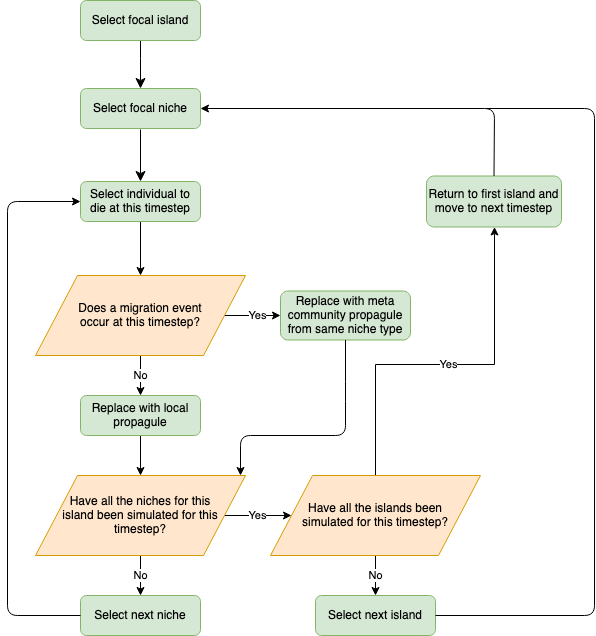
\includegraphics[scale=0.4]{../../Other/neutral_flowchart2.png}
  \caption{Flowchart of simulation design}
  \label{fig:Flowchart}
\end{figure}


\subsubsection{High Performance Computing}
The metacommunity and simulation code are contained in \textit{ClusterSim.R}. \textit{ClusterSim.R} functions are sourced by \textit{ClusterCode.R} and given the input parameters: \textit{J\_meta} = 50000, \textit{nu} = 0.001, \textit{num\_m\_rates} = 20, \textit{max\_k\_num} = 20, \textit{max\_k\_size} = 20, \textit{wall\_time} = 1380, \textit{output\_file\_name} = output\_file\_name (where each simulation is given a unique file name "simulation\_timeseries\_\textit{i}". \textit{ClusterRun.sh} is used to run on the cluster, with a time limit of 24:00:00. \textit{wall\_time} is given as 1380 minutes (23 hours) within the function, to ensure all simulations are completed before the cluster run ends. 100 parallel simulation were run on the Imperial College London High Performance Computing service. This generated a total of 800000 islands, simulated for $>$ 30000 timesteps.   

\subsection{Data Preparation and Timeseries Plots}
The 100 simulation results were imported into \textit{DataPrep.R}. The data from each island was isolated and configured into a data frame with simulation number, migration rate, area, number of niches and number of species (\textit{SimModelFitData.csv}). A second data frame was generated for timeseries plotting, with simulation number, island number, migration rate, timestep and species richness timeseries for each island (\textit{SimTimeseriesPlotData.csv}).\bigskip

\noindent To ensure the simulation had run long enough for each island to reach dynamic equilibrium the species richness timeseries of simulations 25, 50 and 75 were plotted(\textit{TimeseriesPlot.R})(Figure 2).

\subsection{Analysis}\bigskip

\begin{verbatim}
chisholm_model <- function(area, theta, m0, K) {
  rho = 1
  K = K
  Js = area*rho
  J_stars = Js/K
  ms = m0/sqrt(area)
  gamma_stars = J_stars*ms/(1-ms)
  return(theta*(digamma(theta/K+gamma_stars*
  (digamma(gamma_stars+J_stars)-digamma(gamma_stars)))-digamma(theta/K)))
}
\end{verbatim}

\noindent An analysis script (\textit{Analysis.R}) imported the prepared data (\textit{SimModelFitData.csv}) for each island across all simulations (800000 islands). Model estimated species richnesses were generated by giving the island parameters (\textit{m0 = m*sqrt(area)}) and an estimated \textit{theta} (\textit{theta = 2*(niche\_size*K)*nu}, where \textit{niche\_size * K} = size of each niche in the metacommunity from which immigration events can occur times by the number of niches contributing to the island community i.e. number of niches on the island). The results of the simulation and those estimated by the \textit{chisholm\_function} (above) were bound together in a data frame. Mean species richness results for each combination of island area, migration rate and number of niches across all 100 simulations was calculated and stored.


\section{Data Collection and Analysis}

\subsection{Datasets}

\begin{table}[h!]
  \begin{center}
    \caption{Summary of datasets collected from the literature}
    \label{table1}
    \pgfplotstabletypeset[
      multicolumn names, % allows to have multicolumn names
      col sep=comma, % the seperator in our .csv file
      display columns/0/.style={
		column name=$Attribute$, % name of first column
		string type},  % use siunitx for formatting
      display columns/1/.style={
		column name=$Aqua$,
		column type={S},string type},
      display columns/2/.style={
		column name=$Terra$,
		column type={S},string type},
      display columns/3/.style={
		column name=$Total$,
		column type={S},string type},
      every head row/.style={
		before row={\toprule}, % have a rule at top
		after row={
			%\si{\ampere} & \si{\volt}\\ % the units seperated by &
			\midrule} % rule under units
			},
		every last row/.style={after row=\bottomrule}, % rule at bottom
    ]{summary_stats.csv} % filename/path to file
  \end{center}
\end{table}

In-lieu of being able to generate my own dataset, I compiled 36 datasets of microbial species/taxa-area relationships. A full description of each dataset and their authors can be found in the Supplementary Material section. These datasets included a range of taxonomic groups, including archaea, bacteria, fungi, algae, protazoa and pathogens. The datasets also included aquatic and terrestrial habitats, as well as in-situ and lab based investigations. For the majority of datasets, the number of observed species, strains, operational taxonomic units or phylogroups per "island" habitat was taken. Some studies only supplied diversity indexes (gamma diversity, phylogenetic diversity, faiths dp, simpsons index, chao 1, T-RFLP, viral prevalence). The estimated number of cells/individuals per unit area was also taken from each study, or estimated from the relevant literature if unavailable.     

\subsection{Model Fitting}

\begin{equation}
S=\theta\{\psi(\frac{\theta}{K}+\gamma(\psi(\gamma+J)-\psi(\gamma)))-\psi(\frac{\theta}{K})\}
\end{equation} 

For each dataset I found initial parameter estimates for \textit{m} and $\theta$. I then looped through all values of \textit{K} from 1 to the maximum number of taxa recorded on one "island" and fitted the Chisholm model (2.1) using NLLS fitting. From the fitting, the best-fit parameters for \textit{m} and $\theta$ were selected, along with their best fit \textit{K}. On "islands" where the estimated cell count per unit area was less than the value of \textit{K}, estimated species richness was constrained to equal number of individuals so as not to more species than individual microorganisms. %%%is this neccessary???

Values for rho were either taken from the original paper or from the literature.

\subsection{Critical Area}

\begin{equation}
ACrit=\frac{\theta(1 - m)(exp(K/\theta) - 1}{m\rho*log(1/m)}
\end{equation}

For each successful model fitting, the critical area of transition from a niche-structured regime to an extinction-colonisation equilibrium regime was estimated. The best-fit values of \textit{K}, \textit{m} and $\theta$ from the model fitting were given to the critical area equation (2.2). By finding the critical area of regime transition for the datasets, I was able to test the theory that the regime shift would occur at lower areas for "islands" that are less isolated. I then conducted a multiple regression analysis with critical area as dependent variable and habitat type (aquatic/terrestrial) and taxonomic group as categorical variables. 
